\begin{equation}
\Pggx(q) + \Pg(k_1) \rightarrow \PaQ(p_2) + \PQ(p_1)
\end{equation}

\begin{figure}[ht!]
	\centering
	\begin{subfigure}[t]{.4\textwidth}
		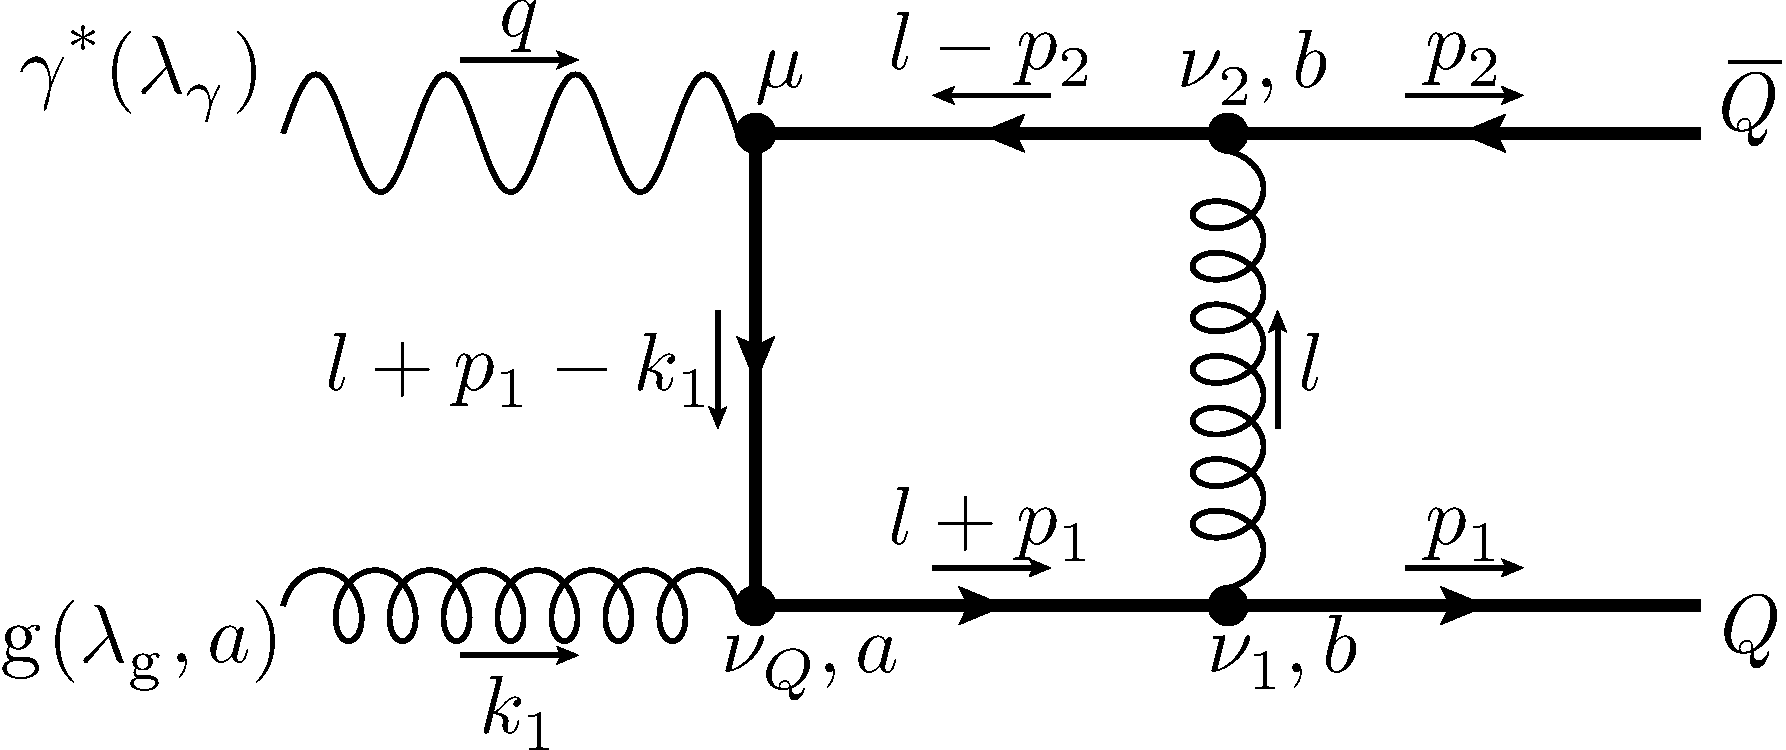
\includegraphics[width=\textwidth]{pyfeyn/nlo-v-box1}
		\caption{$i\Md^{(NLO,v)}_{1,\mu}$}
	\end{subfigure}\hspace{.15\textwidth}%
	\begin{subfigure}[t]{.4\textwidth}
		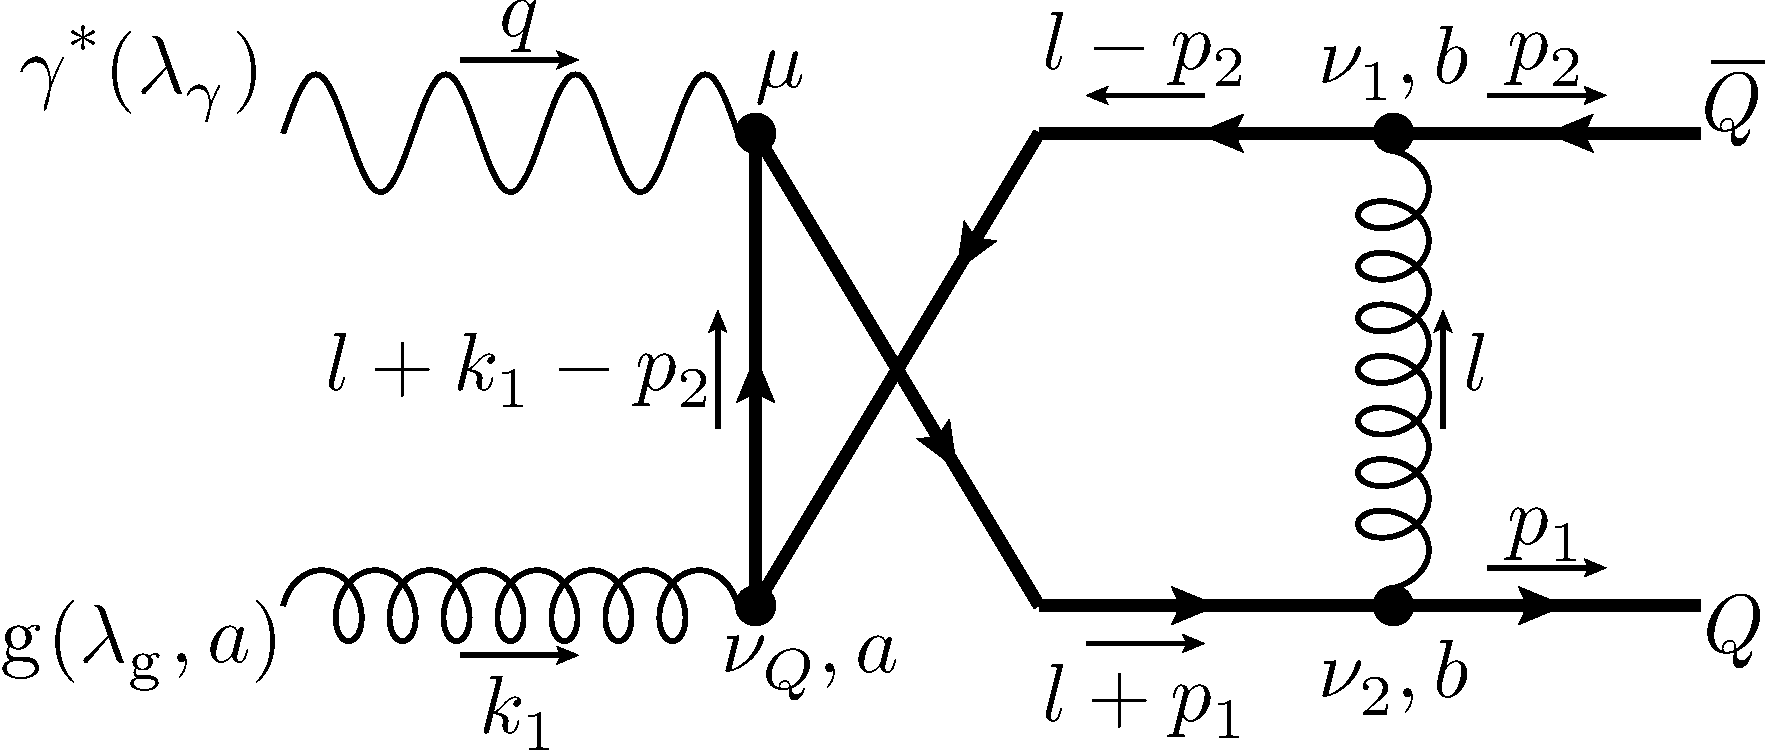
\includegraphics[width=\textwidth]{pyfeyn/nlo-v-box1cr}
		\caption{$i\Md^{(NLO,v)}_{2,\mu}$}
	\end{subfigure}\\
	\begin{subfigure}[t]{.6\textwidth}
		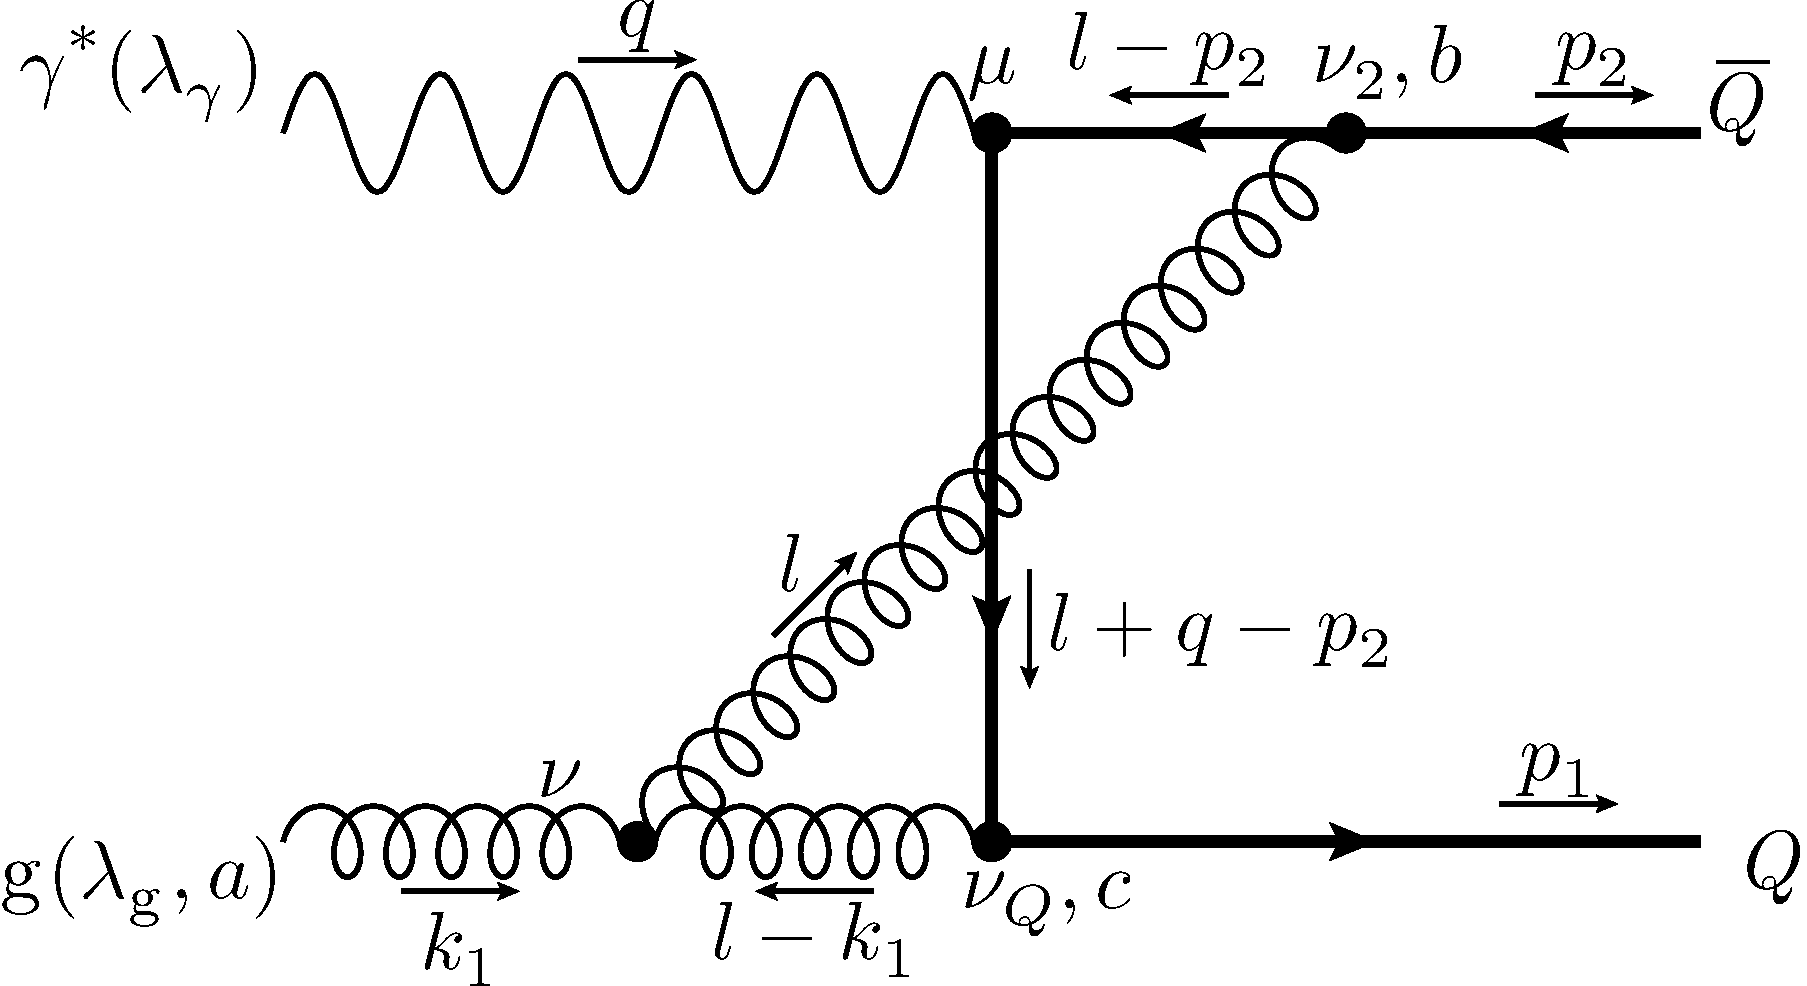
\includegraphics[width=\textwidth]{pyfeyn/nlo-v-box2}
		\caption{$i\Md^{(NLO,v)}_{3,\mu}$}
	\end{subfigure}
	\caption{NLO contributions by one loop}\label{fig:FeynNLOvab}
\end{figure}

\begin{align}
i\Md^{(NLO,v)}_{1,\mu} &=\mu_R^{4-n}\!\!\int\!\!\frac{d^nl}{(2\pi)^n}\,\bar u(p_1)(igT_b\gamma^{\nu_1})\frac{i(\slashed{l}+\slashed{p}_1+m)}{(l+p_1)^2-m^2}(igT_a\gamma^{\nu_Q})\frac{i(\slashed{l}+\slashed{p}_1-\slashed{k}_1+m)}{(l+p_1-k_1)^2-m^2}\cdot\nonumber\\
 &\hspace{40pt}(-i e e_H \gamma_\mu)\frac{i(\slashed{l}-\slashed{p}_2+m)}{(l-p_2)^2-m^2}(igT_b\gamma^{\nu_2})\frac{-ig_{\nu_1,\nu_2}}{l^2}v(p_2)\varepsilon^{(\lambda_{\Pg})}_{\nu_Q}(k_1)\\
i\Md^{(NLO,v)}_{2,\mu} &= \mu_R^{4-n}\!\!\int\!\!\frac{d^nl}{(2\pi)^n}\,\bar u(p_1)(igT_b\gamma^{\nu_1})\frac{i(\slashed{l}+\slashed{p}_1+m)}{(l+p_1)^2-m^2}(igT_a\gamma^{\nu_Q})\frac{i(\slashed{l}+\slashed{p}_1-\slashed{q}+m)}{(l+p_1-q)^2-m^2}\cdot\nonumber\\
 &\hspace{40pt}(-i e e_H \gamma_\mu)\frac{i(\slashed{l}-\slashed{p}_2+m)}{(l-p_2)^2-m^2}(igT_b\gamma^{\nu_2})\frac{-ig_{\nu_1,\nu_2}}{l^2}v(p_2)\varepsilon^{(\lambda_{\Pg})}_{\nu_Q}(k_1)\\
i\Md^{(NLO,v)}_{3,\mu} &=\mu_R^{4-n}\!\!\int\!\!\frac{d^nl}{(2\pi)^n}\,\bar u(p_1)(igT_c\gamma^{\nu_Q})\frac{i(\slashed{l}+\slashed{q}_1-\slashed{p}_2+m)}{(l+q-p_2)^2-m^2}(-i e e_H \gamma_\mu)\frac{i(\slashed{l}-\slashed{p}_2+m)}{(l-p_2)^2-m^2}\cdot\nonumber\\
 &\hspace{20pt}(igT_b\gamma^{\nu_2})\frac{(-i)^2}{l^2(l-k_1)^2}v(p_2)\varepsilon^{\nu,(\lambda_{\Pg})}(k_1)\cdot\nonumber\\
 &\hspace{20pt}\left(gf_{abc}\left(g_{\nu_2\nu_Q}(k_1-2l)_\nu+g_{\nu_Q\nu}(l-2k_1)_{\nu_2}+g_{\nu\nu_2}(k_1+l)_{\nu_Q}\right)\right)
\end{align}

\begin{figure}[ht!]
	\begin{subfigure}[t]{.4\textwidth}
		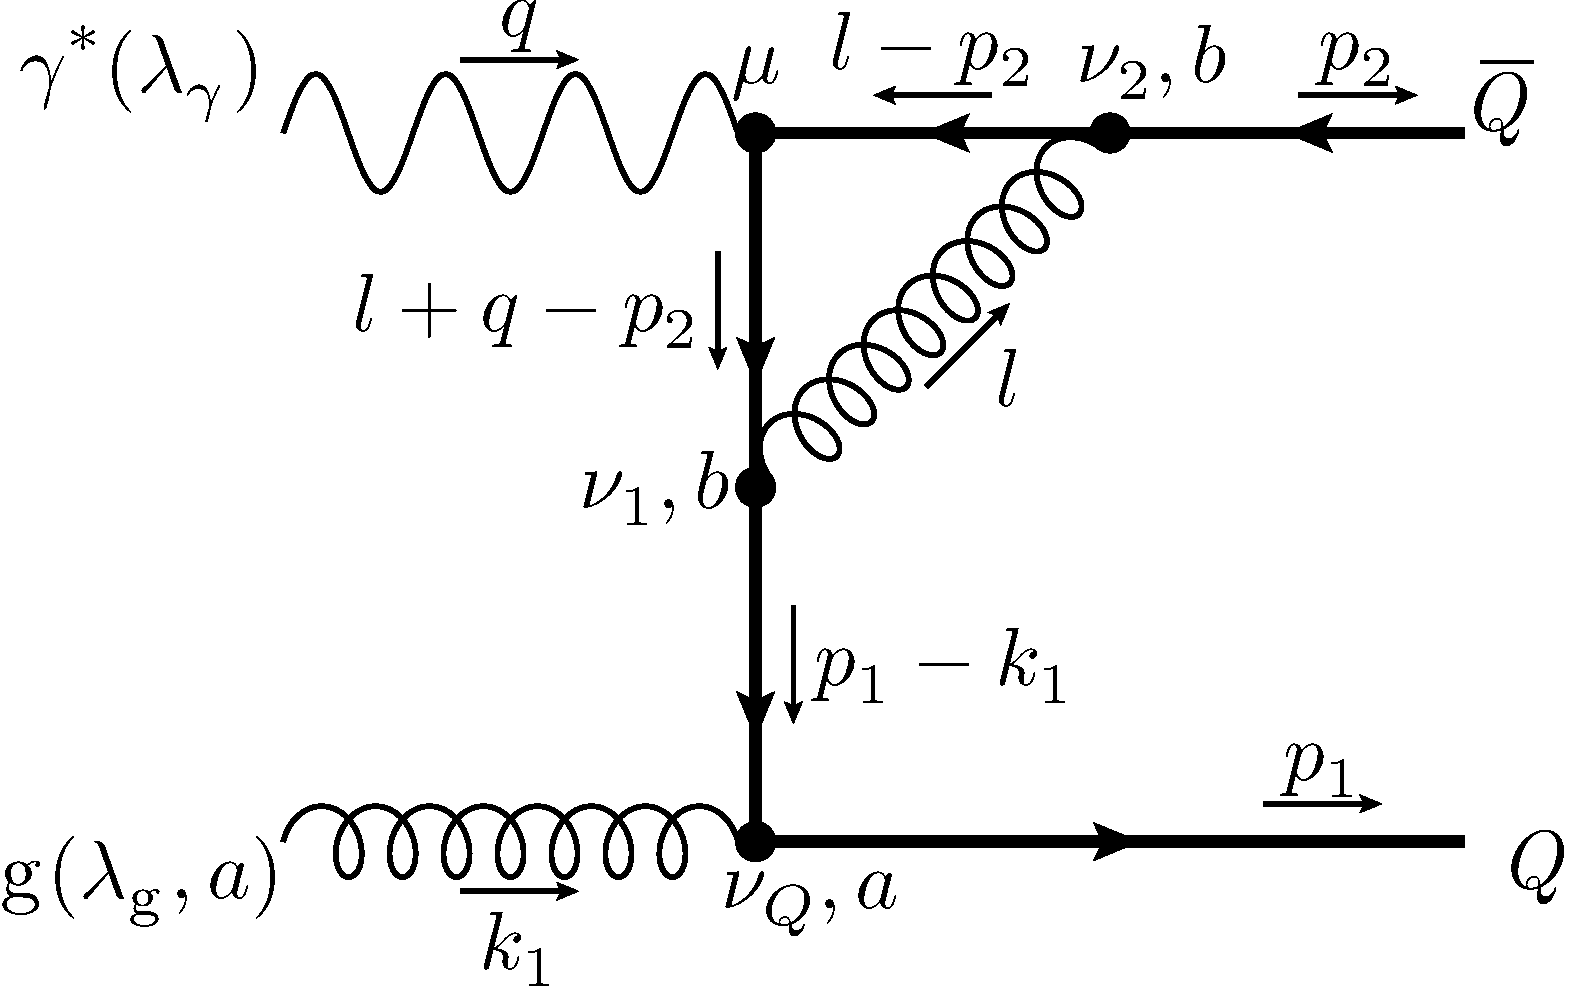
\includegraphics[width=\textwidth]{pyfeyn/nlo-v-e}
		\caption{$i\Md^{(NLO,v)}_{5,\mu}$}
	\end{subfigure}\hspace{.15\textwidth}%
	\begin{subfigure}[t]{.4\textwidth}
		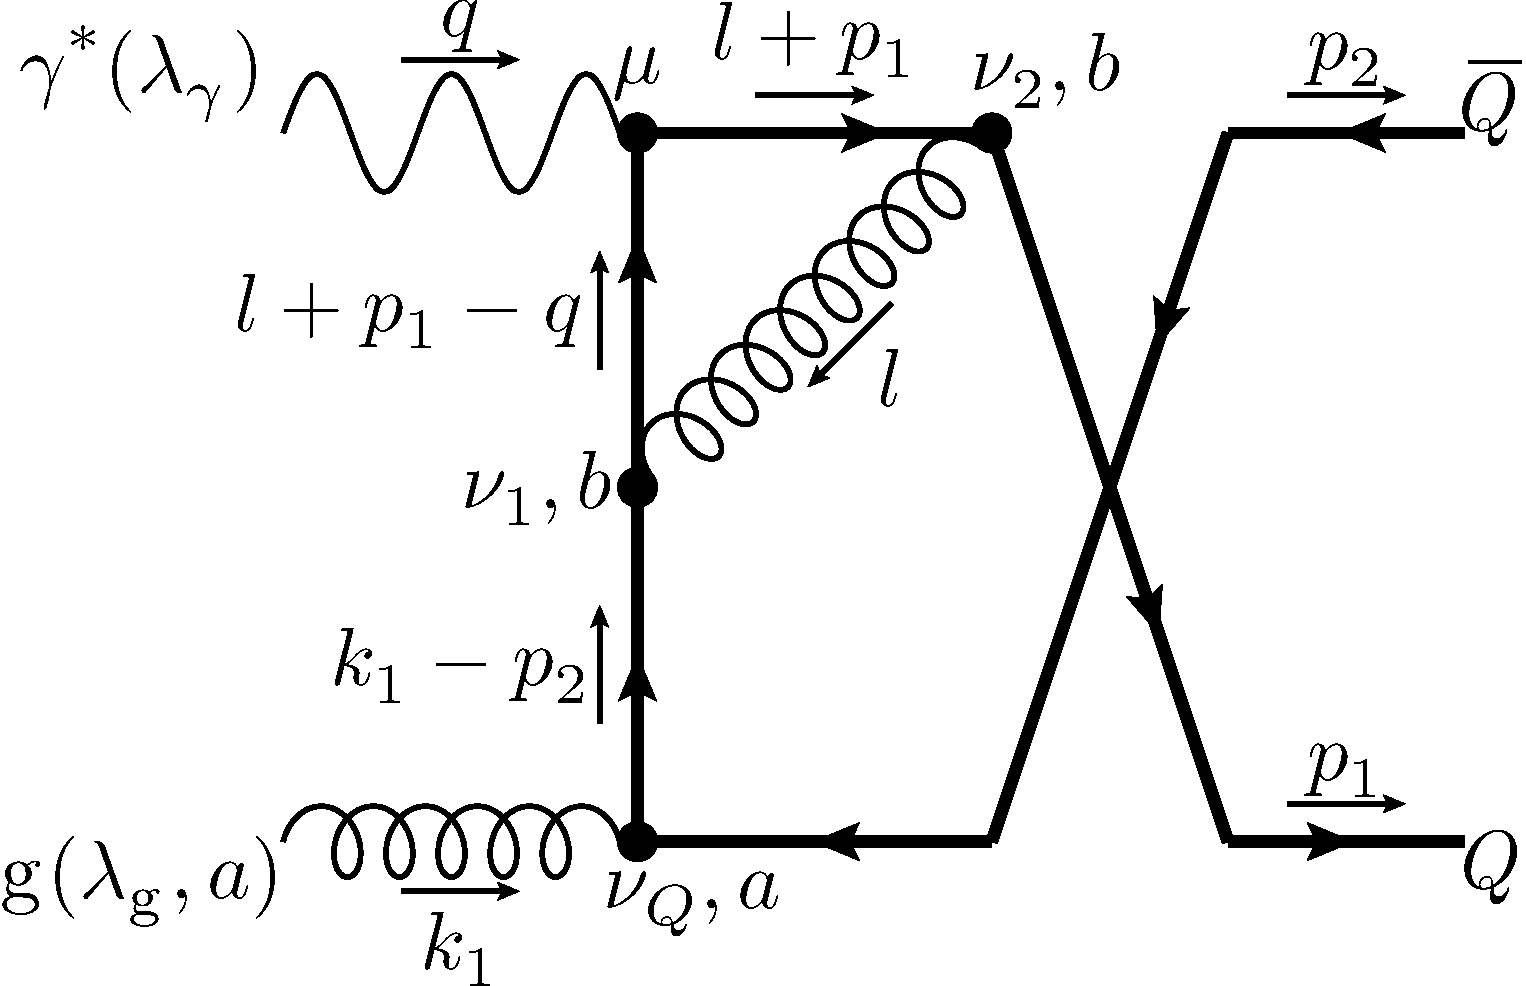
\includegraphics[width=\textwidth]{pyfeyn/nlo-v-ecr}
		\caption{$i\Md^{(NLO,v)}_{6,\mu}$}
	\end{subfigure}\\
	\begin{subfigure}[t]{.4\textwidth}
		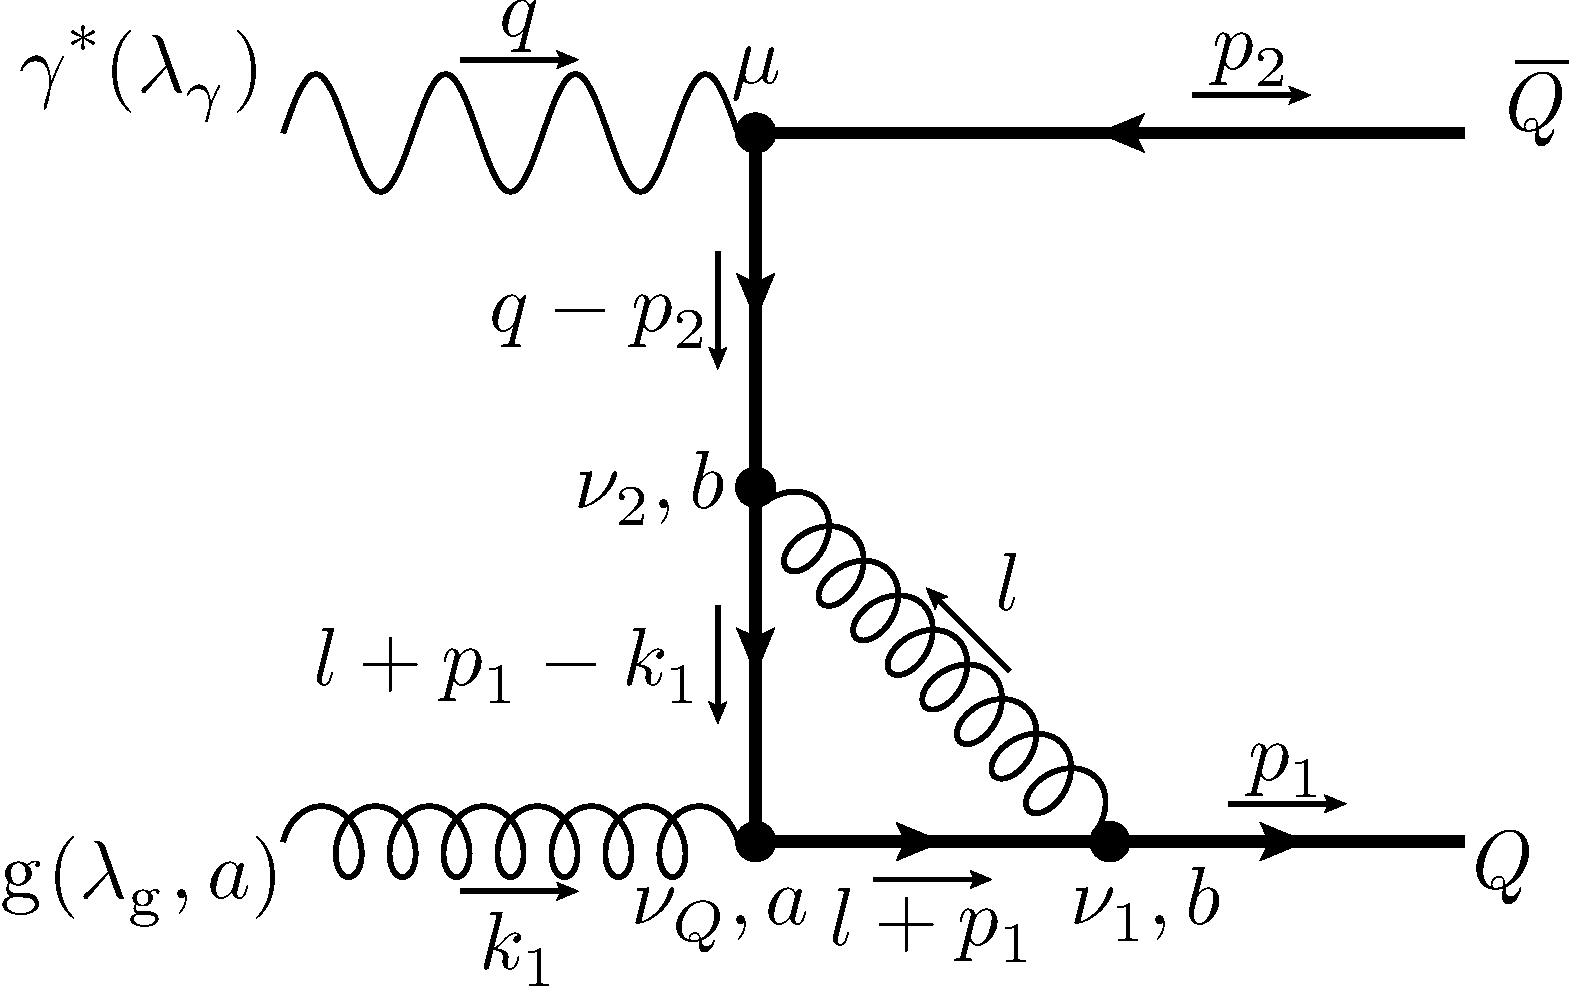
\includegraphics[width=\textwidth]{pyfeyn/nlo-v-g1}
		\caption{$i\Md^{(NLO,v)}_{7,\mu}$}
	\end{subfigure}\hspace{.15\textwidth}%
	\begin{subfigure}[t]{.4\textwidth}
		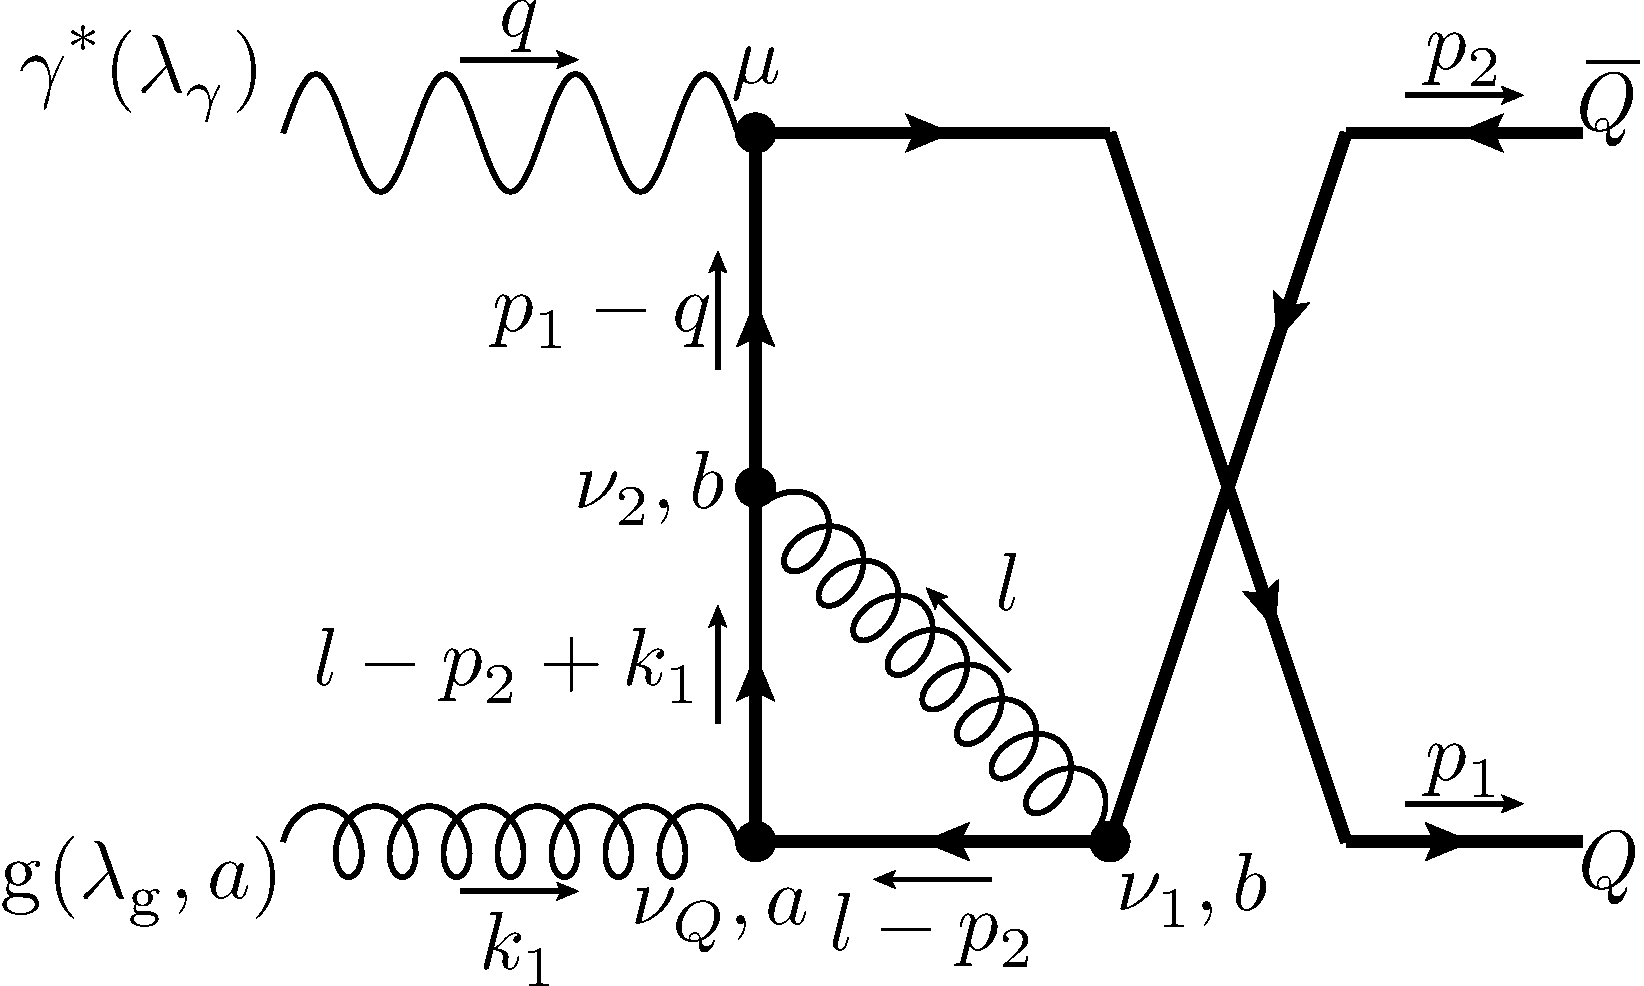
\includegraphics[width=\textwidth]{pyfeyn/nlo-v-g1cr}
		\caption{$i\Md^{(NLO,v)}_{8,\mu}$}
	\end{subfigure}
	\caption{NLO contributions by one loop (cont'ed)}\label{fig:FeynNLOvcd}
\end{figure}

\begin{align}
i\Md^{(NLO,v)}_{5,\mu} &=\mu_R^{4-n}\!\!\int\!\!\frac{d^nl}{(2\pi)^n}\,\bar u(p_1)(igT_a\gamma^{\nu_Q})\frac{i(\slashed{p}_1-\slashed{k}_1+m)}{t_1}(igT_b\gamma^{\nu_1})\frac{i(\slashed{l}+\slashed{q}-\slashed{p}_2+m)}{(l+q-p_2)^2-m^2}\cdot\nonumber\\
 &\hspace{40pt}(-i e e_H \gamma_\mu)\frac{i(\slashed{l}-\slashed{p}_2+m)}{(l-p_2)^2-m^2}(igT_b\gamma^{\nu_2})\frac{-ig_{\nu_1,\nu_2}}{l^2}v(p_2)\varepsilon^{(\lambda_{\Pg})}_{\nu_Q}(k_1)\\
i\Md^{(NLO,v)}_{6,\mu} &=\mu_R^{4-n}\!\!\int\!\!\frac{d^nl}{(2\pi)^n}\,\bar u(p_1)(igT_b\gamma^{\nu_2})\frac{i(\slashed{l}+\slashed{p}_1+m)}{(l+p_1)^2-m^2}(-i e e_H \gamma_\mu)\frac{i(\slashed{l}+\slashed{p}_1-\slashed{q}+m)}{(l+p_1-q)^2-m^2}\cdot\nonumber\\
 &\hspace{40pt}(igT_b\gamma^{\nu_1})\frac{i(\slashed{k}_1-\slashed{p}_2+m)}{u_1}(igT_a\gamma^{\nu_Q})\frac{-ig_{\nu_1,\nu_2}}{l^2}v(p_2)\varepsilon^{(\lambda_{\Pg})}_{\nu_Q}(k_1)\\
i\Md^{(NLO,v)}_{7,\mu} &=\mu_R^{4-n}\!\!\int\!\!\frac{d^nl}{(2\pi)^n}\,\bar u(p_1)(igT_b\gamma^{\nu_1})\frac{i(\slashed{l}+\slashed{p}_1+m)}{(l+p_1)^2-m^2}(igT_a\gamma^{\nu_Q})\frac{i(\slashed{l}+\slashed{p}_1-\slashed{k}_1+m)}{(l+p_1-k_1)^2-m^2}\cdot\nonumber\\
 &\hspace{40pt}(igT_b\gamma^{\nu_2})\frac{i(\slashed{q}-\slashed{p}_2+m)}{t_1}(-i e e_H \gamma_\mu)\frac{-ig_{\nu_1,\nu_2}}{l^2}v(p_2)\varepsilon^{(\lambda_{\Pg})}_{\nu_Q}(k_1)\\
i\Md^{(NLO,v)}_{8,\mu} &=\mu_R^{4-n}\!\!\int\!\!\frac{d^nl}{(2\pi)^n}\,\bar u(p_1)(-i e e_H \gamma_\mu)\frac{i(\slashed{p}_1-\slashed{q}+m)}{u_1}(igT_b\gamma^{\nu_2})\frac{i(\slashed{l}-\slashed{p}_2+\slashed{k}_1+m)}{(l-p_2+k_1)^2-m^2}\cdot\nonumber\\
 &\hspace{40pt}(igT_a\gamma^{\nu_Q})\frac{i(\slashed{l}-\slashed{p}_2+m)}{(l-p_2)^2-m^2}(igT_b\gamma^{\nu_1})\frac{-ig_{\nu_1,\nu_2}}{l^2}v(p_2)\varepsilon^{(\lambda_{\Pg})}_{\nu_Q}(k_1)
\end{align}

\begin{figure}[ht!]
	\begin{subfigure}[t]{.4\textwidth}
		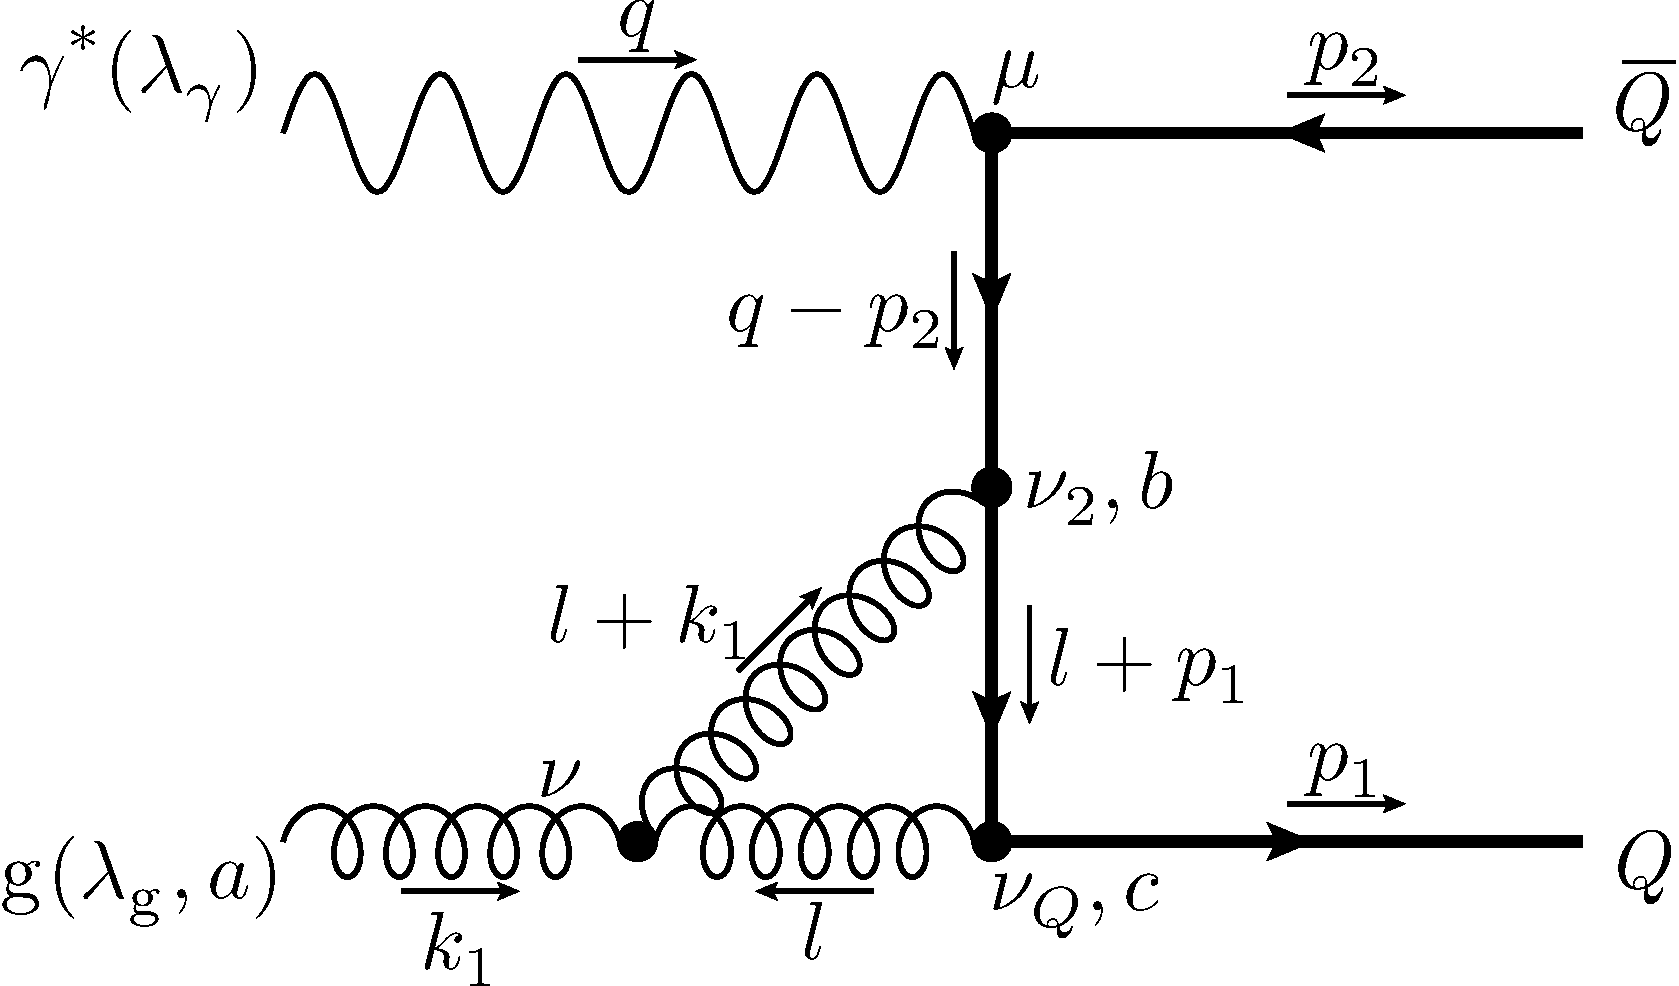
\includegraphics[width=\textwidth]{pyfeyn/nlo-v-g2}
		\caption{$i\Md^{(NLO,v)}_{9,\mu}$}
	\end{subfigure}\hspace{.15\textwidth}%
	\begin{subfigure}[t]{.4\textwidth}
		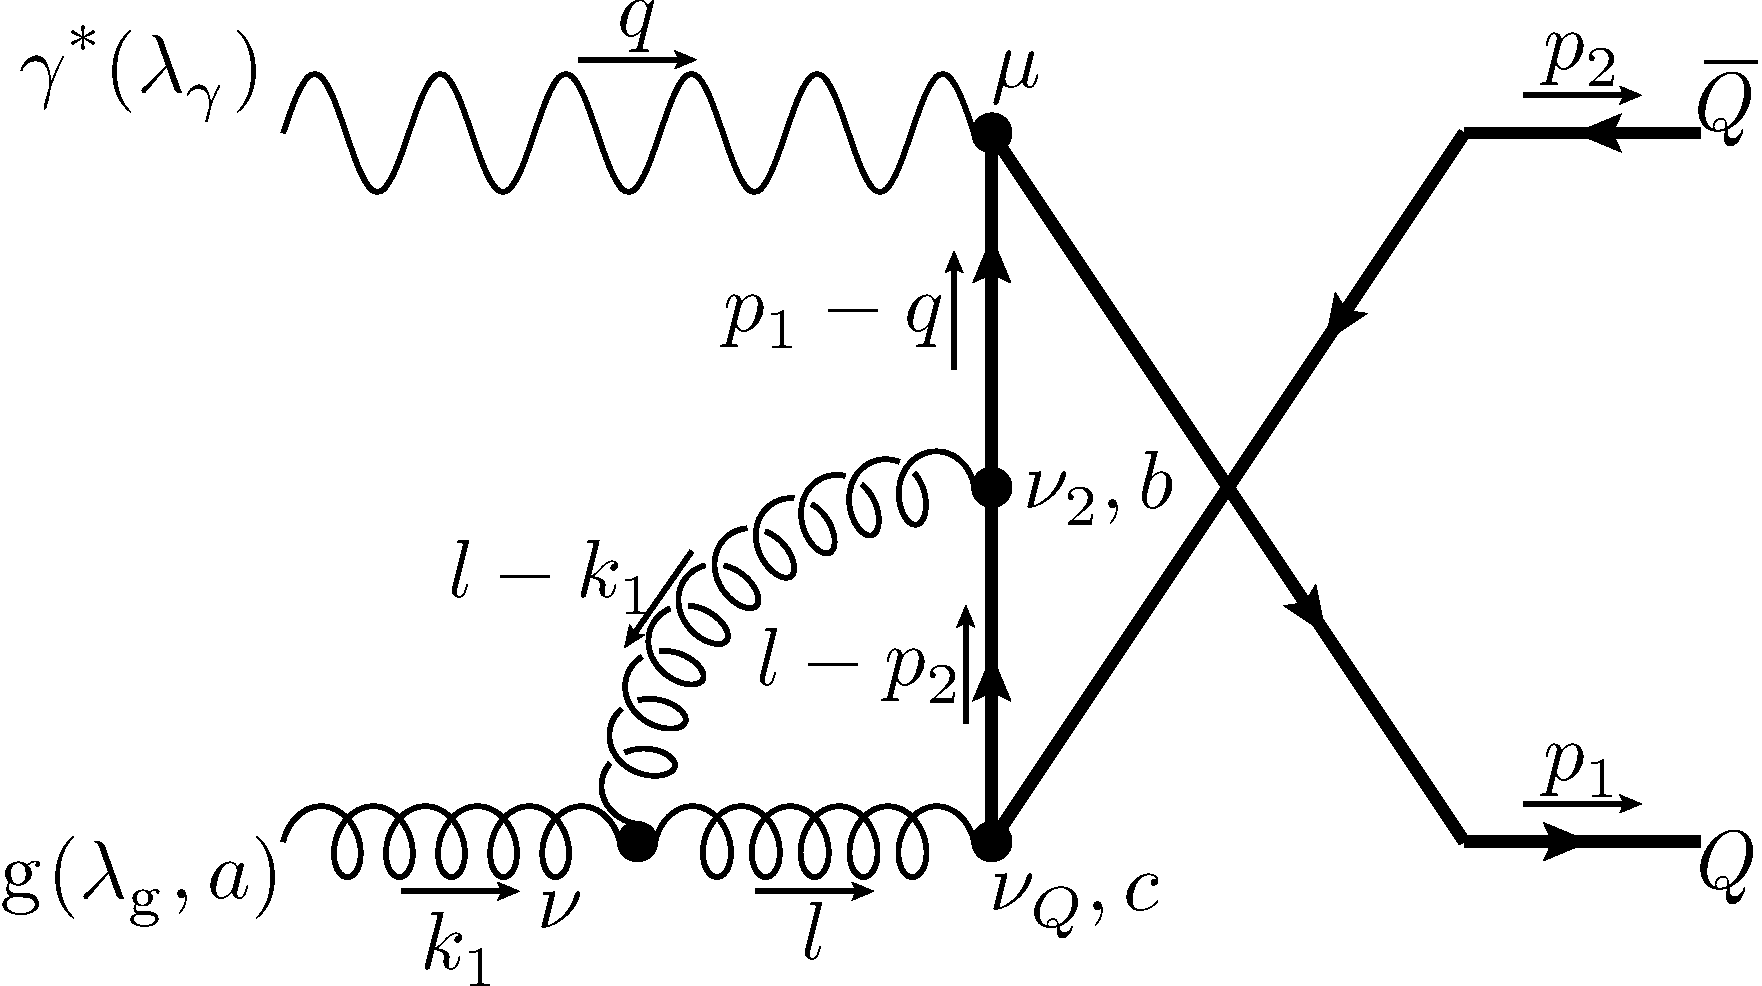
\includegraphics[width=\textwidth]{pyfeyn/nlo-v-g2cr}
		\caption{$i\Md^{(NLO,v)}_{10,\mu}$}
	\end{subfigure}\\
	\begin{subfigure}[t]{.4\textwidth}
		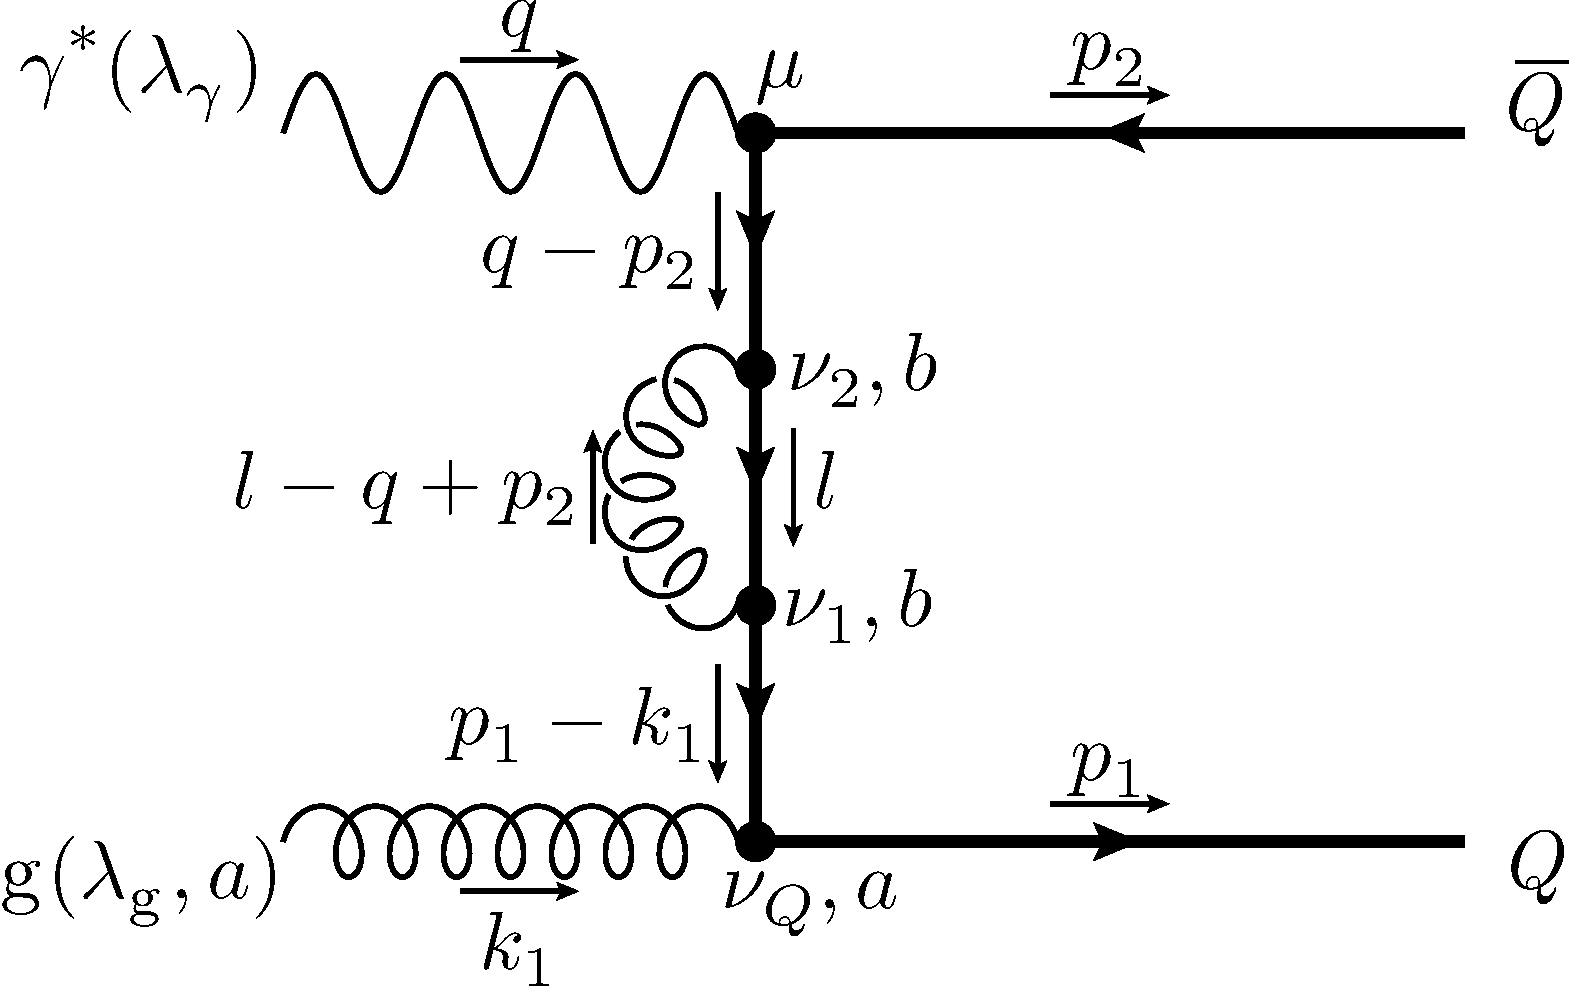
\includegraphics[width=\textwidth]{pyfeyn/nlo-v-m1}
		\caption{$i\Md^{(NLO,v)}_{11,\mu}$}
	\end{subfigure}\hspace{.15\textwidth}%
	\begin{subfigure}[t]{.4\textwidth}
		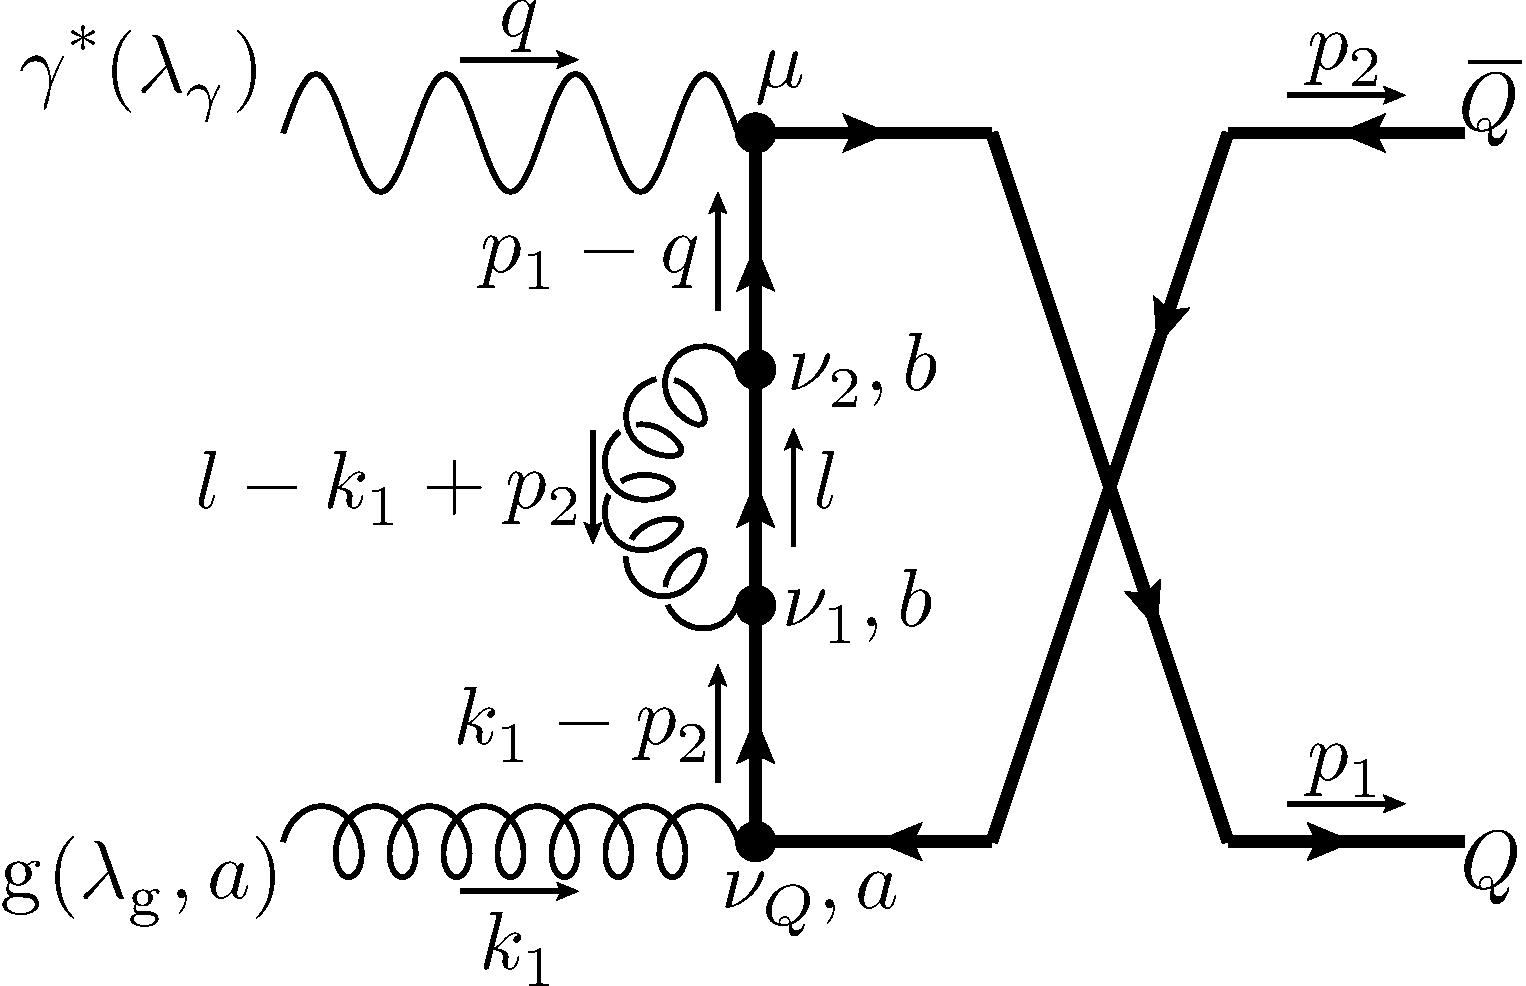
\includegraphics[width=\textwidth]{pyfeyn/nlo-v-m1cr}
		\caption{$i\Md^{(NLO,v)}_{12,\mu}$}
	\end{subfigure}
	\caption{NLO contributions by one loop (cont'ed)}\label{fig:FeynNLOvef}
\end{figure}

\begin{align}
i\Md^{(NLO,v)}_{9,\mu} &=\mu_R^{4-n}\!\!\int\!\!\frac{d^nl}{(2\pi)^n}\,\bar u(p_1)(igT_c\gamma^{\nu_Q})\frac{i(\slashed{l}+\slashed{p}_1+m)}{(l+p_1)^2-m^2}(igT_b\gamma^{\nu_2})\frac{i(\slashed{q}-\slashed{p}_2+m)}{t_1}\cdot\nonumber\\
 &\hspace{20pt}(-i e e_H \gamma_\mu)\frac{(-i)^2}{l^2(l+k_1)^2}v(p_2)\varepsilon^{\nu,(\lambda_{\Pg})}(k_1)\cdot\nonumber\\
 &\hspace{20pt}\left(gf_{abc}\left(g_{\nu\nu_2}(2k_1+l)_{\nu_Q}+g_{\nu_2\nu_Q}(-2l-k_1)_{\nu}+g_{\nu_Q\nu}(l-k_1)_{\nu_2}\right)\right)\\
i\Md^{(NLO,v)}_{10,\mu} &=\mu_R^{4-n}\!\!\int\!\!\frac{d^nl}{(2\pi)^n}\,\bar u(p_1)(-i e e_H \gamma_\mu)\frac{i(\slashed{p}_1-\slashed{q}+m)}{u_1}(igT_b\gamma^{\nu_2})\frac{i(\slashed{l}-\slashed{p}_2+m)}{(l-p_2)^2-m^2}\cdot\nonumber\\
 &\hspace{20pt}(igT_c\gamma^{\nu_Q})\frac{(-i)^2}{l^2(l-k_1)^2}v(p_2)\varepsilon^{\nu,(\lambda_{\Pg})}(k_1)\cdot\nonumber\\
 &\hspace{20pt}\left(gf_{abc}\left(g_{\nu\nu_2}(2k_1-l)_{\nu_Q}+g_{\nu_2\nu_Q}(2l-k_1)_{\nu}+g_{\nu_Q\nu}(-l-k_1)_{\nu_2}\right)\right)\\
i\Md^{(NLO,v)}_{11,\mu} &=\mu_R^{4-n}\!\!\int\!\!\frac{d^nl}{(2\pi)^n}\,\bar u(p_1)(igT_a\gamma^{\nu_Q})\frac{i(\slashed{p}_1-\slashed{k}_1+m)}{t_1}(igT_b\gamma^{\nu_1})\frac{i(\slashed{l}+m)}{l^2-m^2}\cdot\nonumber\\
 &\hspace{40pt}(igT_b\gamma^{\nu_2})\frac{i(\slashed{q}-\slashed{p}_2+m)}{t_1}(-i e e_H \gamma_\mu)\frac{-ig_{\nu_1,\nu_2}}{(l-q+p_2)^2}v(p_2)\varepsilon^{(\lambda_{\Pg})}_{\nu_Q}(k_1)\\
i\Md^{(NLO,v)}_{12,\mu} &=\mu^{4-n}\!\!\int\!\!\frac{d^nl}{(2\pi)^n}\,\bar u(p_1)(-i e e_H \gamma_\mu)\frac{i(\slashed{p}_1-\slashed{q}+m)}{u_1}(igT_b\gamma^{\nu_2})\frac{i(\slashed{l}+m)}{l^2-m^2}\cdot\nonumber\\
 &\hspace{40pt}(igT_b\gamma^{\nu_1})\frac{i(\slashed{k}_1-\slashed{p}_2+m)}{u_1}(igT_a\gamma^{\nu_Q})\frac{-ig_{\nu_1,\nu_2}}{(l-k_1+p_2)^2}v(p_2)\varepsilon^{(\lambda_{\Pg})}_{\nu_Q}(k_1)
\end{align}

color space:
\begin{align}
\left(\Md^{(NLO,v)}_{1,\mu}+\Md^{(NLO,v)}_{2,\mu}\right)\left(\Md^{(LO)}_{1,\mu'}+\Md^{(LO)}_{2,\mu'}\right)^*&\sim -i\tr(T_aT_bT_aT_b) = -iN_C C_F \left(C_F - \frac{C_A}{2}\right)\\
\left(\Md^{(NLO,v)}_{3,\mu}\right)\left(\Md^{(LO)}_{1,\mu'}+\Md^{(LO)}_{2,\mu'}\right)^*&\sim f_{abc}\tr(T_cT_bT_a) = -\frac i 2 N_C C_F C_A\\
\left(\Md^{(NLO,v)}_{5,\mu}+\Md^{(NLO,v)}_{6,\mu}\right)\left(\Md^{(LO)}_{1,\mu'}+\Md^{(LO)}_{2,\mu'}\right)^*&\sim -i\tr(T_aT_aT_bT_b) = -iN_C C_F^2\\
\end{align}

to compute self energies, we follow \cite{Bojak:2000eu}.
It is
\begin{align}
\{\gamma_\mu,\gamma_\nu\} &= 2g_{\mu\nu}\\
\gamma_\mu\gamma^\mu &= g_\mu^\mu = n \\
\gamma_\mu\gamma_\nu\gamma^\mu &= (2-n)\gamma_\nu
\end{align}
\begin{figure}[ht!]
	\begin{subfigure}[t]{.4\textwidth}
		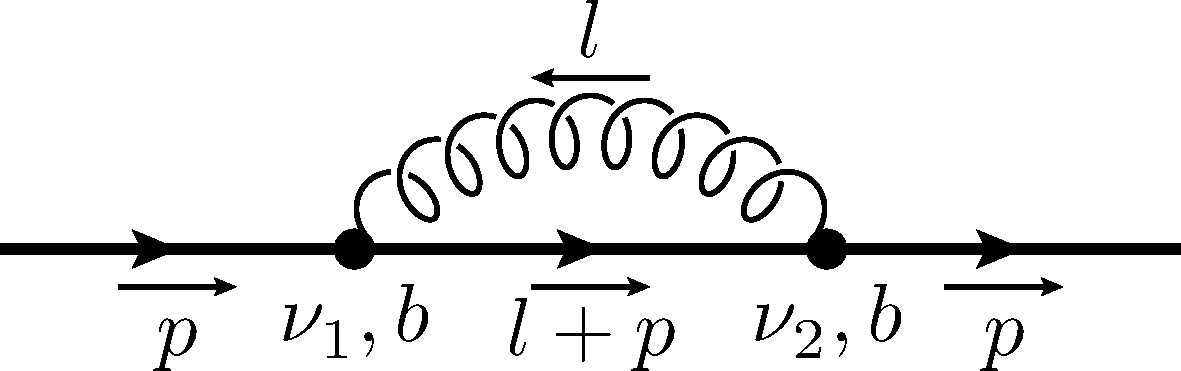
\includegraphics[width=\textwidth]{pyfeyn/nlo-v-seq}
		\caption{$-i\Sigma(p)$}
	\end{subfigure}\hspace{.15\textwidth}%
	\begin{subfigure}[t]{.4\textwidth}
		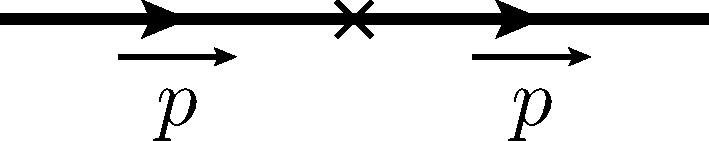
\includegraphics[width=\textwidth]{pyfeyn/nlo-v-seqc}
		\caption{$-i\Sigma_C(p)$}
	\end{subfigure}
	\caption{NLO contributions by quark self energy}\label{fig:FeynNLOvseq}
\end{figure}
\begin{align}
-i\Sigma(p) &= \mu_R^{4-n}\!\!\int\!\!\frac{d^nl}{(2\pi)^n}(igT_b \gamma_{\nu_1})\frac{i(\slashed{l}+\slashed{p}+m)}{(l+p)^2-m^2}(igT_b \gamma_{\nu_2})\frac{-ig^{\nu_1,\nu_2}}{l^2}\\
 &=-\mu_R^{4-n}g^2C_F\!\!\int\!\!\frac{d^nl}{(2\pi)^n}\frac{2m+(2-n)\slashed{p}+(2-n)\slashed{l}}{l^2((l+p)^2-m^2)}\\
 &=-g^2C_F\left(\left(2m+(2-n)\slashed{p}\right)B_0(p^2,0,m^2)+(2-n)B_1(p^2,0,m^2)\right)\\
 &=-g^2C_F\left(B_0(p^2,0,m^2)\left(n\cdot m+(2-n)\slashed{p}\frac{p^2+m^2}{2p^2}\right)-(2-n)\slashed{p}\frac 1{2p^2}A_0(m^2)\right)
\end{align}
Using \cite{Bojak:2000eu} we find
\begin{align}
C_\epsilon &= \frac 1 {16\pi^2}\exp\left(\left(\gamma_E-\log(4\pi)\right)\frac{\epsilon} 2\right)\left(m^2/\mu^2\right)^{\epsilon/2}\\
A_0(m^2) &=iC_\epsilon\left(-\frac 2 {\epsilon}+1\right)\\
B_0(p^2,0,m^2) &=iC_\epsilon\left(-\frac 2{\epsilon}+2+\frac{m^2-p^2}{p^2}\ln\left(\frac{m^2-p^2}{m^2}\right)\right)
\end{align}
\begin{align}
\Rightarrow-i\Sigma(p) &= -ig^2C_FC_\epsilon\left[\frac{2\slashed{p}-8m}{\epsilon}+2m\left(3-2\left(1-\frac{m^2}{p^2}\right)\ln\left(1-\frac{p^2}{m^2}\right)\right)\right.\nonumber\\
 &\hspace{90pt}\left.-\slashed{p}\left(1+\frac{m^2}{p^2}\right)\left(1-\left(1-\frac{m^2}{p^2}\right)\ln\left(1-\frac{p^2}{m^2}\right)\right)\right]\\
 &\EqualClaim -i(A m + B(\slashed p - m))
\end{align}
\begin{align}
\Rightarrow A &= \frac 1 m \left.\Sigma(p)\right|_{\slashed{p}=m} \\
 &= -g^2C_F C_\epsilon\left(\frac 6 \epsilon -5 +\frac{m^2}{p^2}+\left(3-4\frac{m^2}{p^2}+\frac{m^4}{p^4}\right)\ln\left(1-\frac{p^2}{m^2}\right)\right)\\
\Rightarrow B &= \frac 1 m \left.\DeriveF{\slashed{p}}{\Sigma(p)}\right|_{\slashed{p}=m} \\
 &= g^2C_F C_\epsilon\left(\frac 2 \epsilon -1-\frac{m^2}{p^2}+\left(1-\frac{m^4}{p^4}\right)\ln\left(1-\frac{p^2}{m^2}\right)\right)
\end{align}

Counterterm:
\begin{align}
-i\Sigma_C(p) &=i((Z_2-1)\slashed{p}-(Z_2 Z_m -1) m)\\
 &= i((Z_2-1)(\slashed p - m) - (Z_m-1)m) + O(\alpha_S^2)
\end{align}

Use on-shell renormalisation:
\begin{align}
0 &\EqualClaim \left.\left(-i\Sigma(p)-i\Sigma_C(p)\right)\right|_{\slashed{p}=m}\\
 &= i(((Z_m-1)+A)m+(B-(Z_2-1))(\slashed p - m)) \\
\Rightarrow (Z_m-1) &= \left.-A\right|_{\slashed{p}=m}\\
 &= g^2C_F C_\epsilon\left(\frac 6 \epsilon -4\right)
\end{align}
